\documentclass{article}

\usepackage[left=1in, right=1in, top=1in, bottom=1in]{geometry}

\usepackage{setspace}
\usepackage{fancyhdr}
\usepackage{hyperref}
\usepackage{amsthm}
\usepackage{amssymb}
\usepackage{multirow}
\usepackage{enumitem}
\usepackage{graphicx}
\usepackage{makecell}
\usepackage{booktabs}
\usepackage{titlesec}
\usepackage{amsmath}
\usepackage{pdfpages}
\usepackage{enumitem}
\usepackage{caption}


\setcounter{secnumdepth}{4}

\hypersetup{
    colorlinks=true,     
    urlcolor=cyan
}

\renewcommand{\qedsymbol}{\rule{0.7em}{0.7em}}

\newlength\tindent
\setlength{\tindent}{\parindent}
\setlength{\parindent}{0pt}
\renewcommand{\indent}{\hspace*{\tindent}}
\setlength{\parskip}{0em}

\newenvironment{blockquote}{%
  \par%
  \vskip1em
  \leftskip=2em\rightskip=2em%
  \noindent\ignorespaces}{%
  \par\vskip1em}

\newenvironment{blockquote2}{%
	\par%
	\vskip1em
	\leftskip=4em\rightskip=4em%
	\noindent\ignorespaces}{%
	\par\vskip1em}

\pagestyle{fancy}
\fancyhf{}
\fancyhead[LO]{STA5176}
\fancyhead[RO]{Kyle Ligon}
\fancyfoot[LO]{Final Project}
\fancyfoot[RO]{\thepage}
 
\renewcommand{\headrulewidth}{0.5pt}
\renewcommand{\footrulewidth}{0.5pt}

\begin{document}
\section*{Final Project}
\section*{Due 4-27-2018}
\subsection*{Introduction}

\indent Baltimore, Maryland, just the name of the city brings to mind countless forms of illegality and the varied levels of force spent to counteract such actions.  Whether it be the spike in recent carjackings from 2017 and the judicial systems lax consequences against the youth committing the crimes or Freddie Grey's death in the back seat of a police van after not being secured by officers after his arrest for possession of an illegal knife, Baltimore remains a city centered on the yin and yang between crimes committed and the response to those crimes.  To help people better understand the Baltimore's crime as well as add transparency to what police officers are up against, the Baltimore Police Department released crime statistics going back to December 2011.  The statistics are open for interaction in many ways including downloading as a .csv file, visualizing through plot.ly, and access through a SODA API.  In addition, this dataset was made available on kaggle.com for kernels to be produced on the data.  The goal of this project is better understand the behaviors associated with many different types of crimes in the city of Baltimore.  

\subsection*{Methods}

\indent The data was downloaded as a .csv file from \url{https://www.kaggle.com/sohier/crime-in-baltimore} and read into R for analysis.  Upon inspection, the data set contained crime and arrest records back to 12/15/2011.  The set is 276,529 rows of 15 columns including: CrimeDate, Location, Description, Inside/Outside, District, Neighborhood, and Total Incidents.  A little bit of exploratory data analysis was done to spur the questions the following hypotheses attempt to answer.  Finally, F tests were used to determine relationships of variance as well as whether variances were equal in mean tests.  T-tests were used to determine differences or equality of means after checking equality of variances.  If the equal variances requirement was violated, a Wilcoxon rank sum test was used.  In comparing percents, a two proportion z test was used to determine differences.  Finally, in looking at multiple means, an ANOVA was used to check differences with a Tukey HSD determining which pairs were significantly different.    

\begin{figure}[h]
\centering
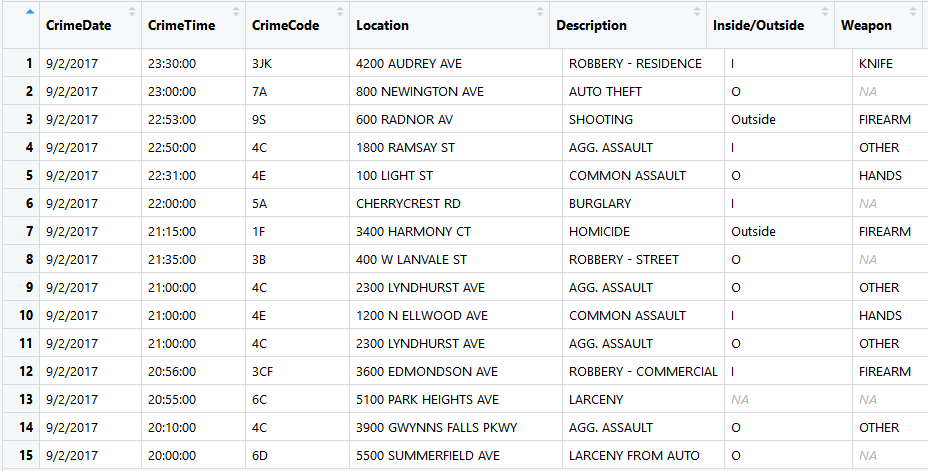
\includegraphics[width = 1.0\textwidth]{DataSetView.png}
\end{figure}


\subsection*{Hypotheses}
\indent  \textbf{Test 1:} Are the number of Arsons committed in one month more varied in the Winter months (December, January, and February) in comparison to the other nine months?

$H_{0}: \sigma_{Winter}^{2} = \sigma_{SprSumWin}^{2}$ \\
$H_{1}: \sigma_{Winter}^{2} > \sigma_{SprSumWin}^{2}$ \\

\indent \textbf{Test 2:} Are there more Auto Thefts on Weekends over Weekdays?

$H_{0}: \mu_{Weekend} = \mu_{Weekday}$ \\
$H_{1}: \mu_{Weekend} = \mu_{Weekday}$ \\

\indent \textbf{Test 3:} On a given night are there more shootings inside a residence than outside?  

$H_{0}: M_{Inside} = M_{Outside}$ \\
$H_{1}: M_{Inside} > M_{Outside}$ \\

\indent \textbf{Test 4:} On any given day, if you are assaulted, is it more likely to be a common assault?  

$H_{0}: \mu_{CommonAssault} = \mu_{AggAssault}$ \\
$H_{1}: \mu_{CommonAssault} > \mu_{AggAssault}$ \\

\indent \textbf{Test 5:} Is there a district with a distinctly higher number of Burglary's in the Summer months?  If so, which are significantly different?  

$H_{0}: \mu_{Central} = \mu_{Eastern} = \mu_{Northeastern} = \mu_{Northern} = \mu_{Northwestern} = \mu_{Southeastern} = \mu_{Southern} = \mu_{Southwestern} = \mu_{Western}$ \\
$H_{1}:$ At least one mean is different.  \\

\subsection*{Conclusion}
\indent With so much data within this data set, this analysis hardly counts as a tip of the iceberg in identifying relationships between Crime(s) in Baltimore.  Going forward, an in depth look at how all of these different crimes have changed over time would help shed some light on where Baltimore is seeing a decrease 



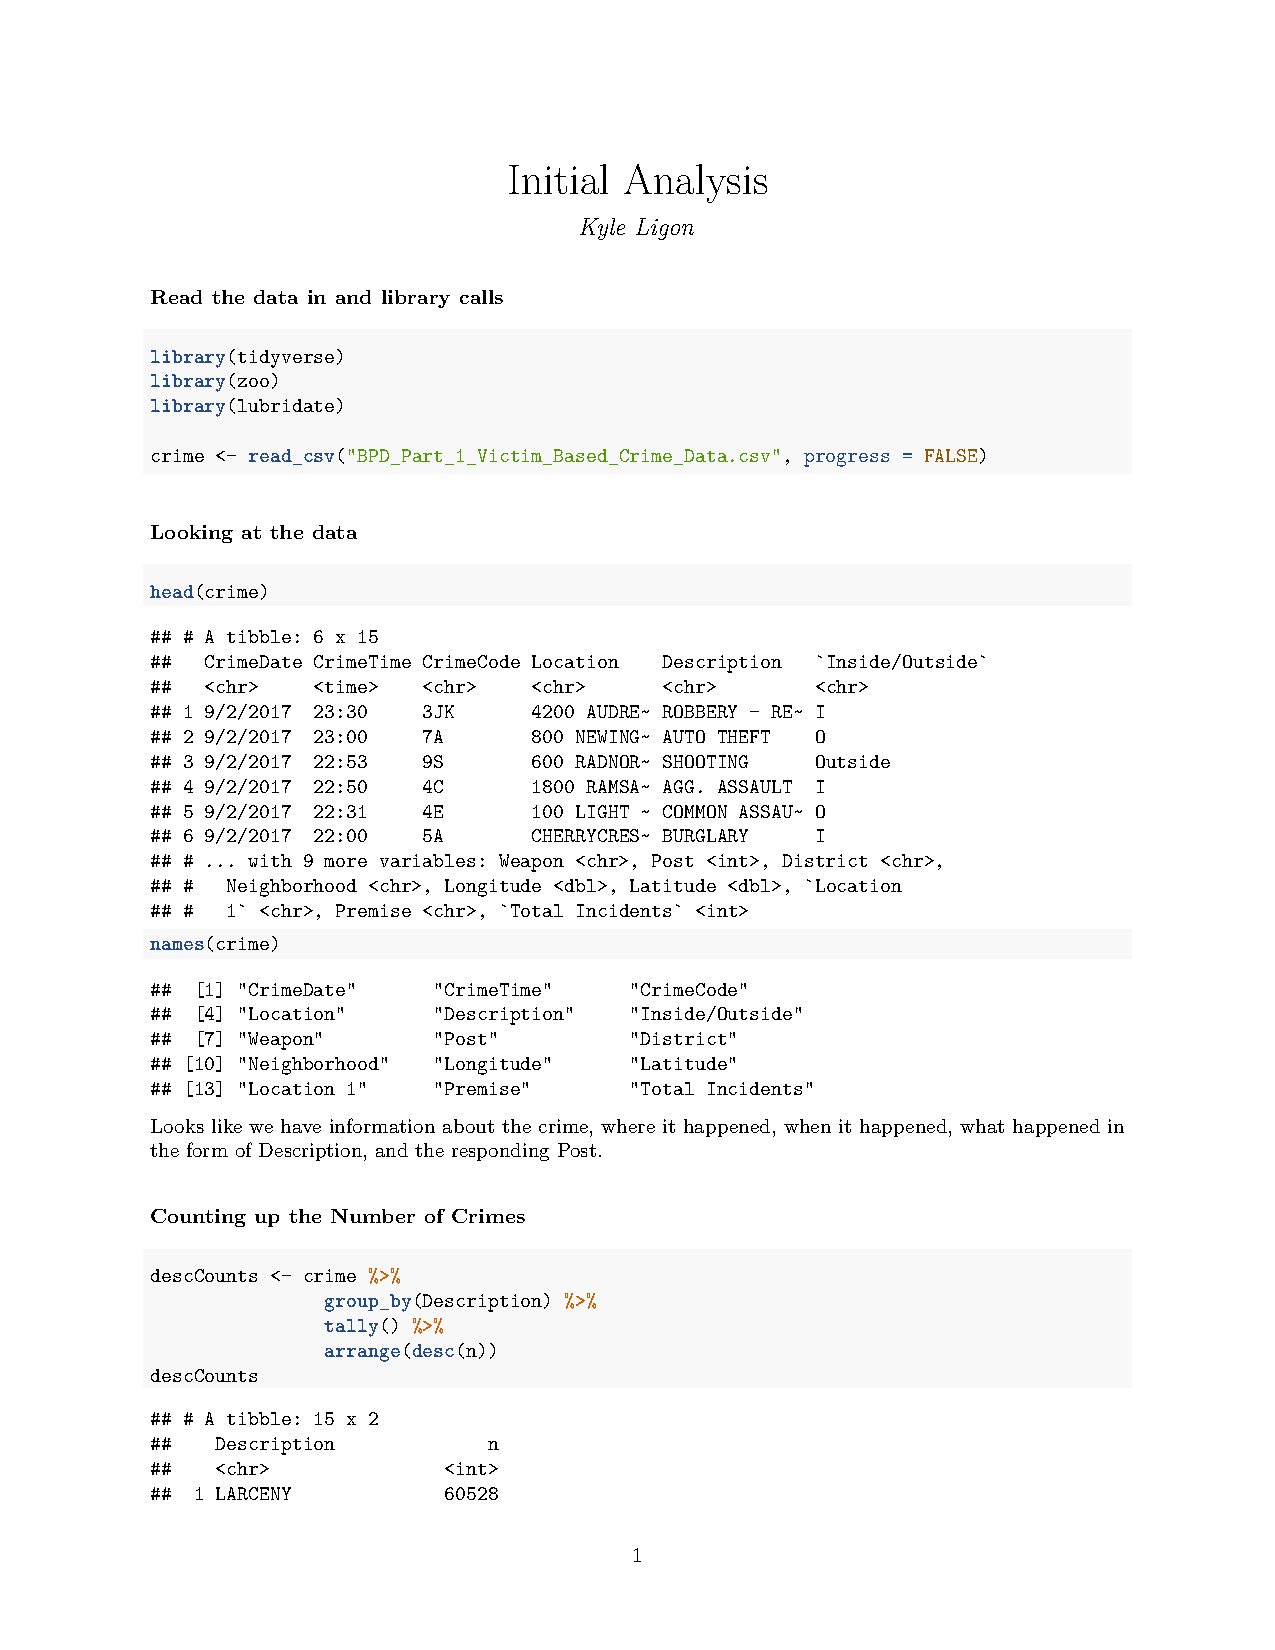
\includepdf[pages=-]{EDA_Notebook.pdf}

\end{document}